\chapter{Implementación}
\label{chapter:implementacion}

Este capítulo describe la implementación del modelo de \citeauthor{echeveste2020cortical} dentro del framework Scikit-NeuroMSI. La implementación abarca desde la arquitectura de software hasta los algoritmos de optimización, pasando por el modelo generativo \acrshort{GSM}, las dinámicas de la red \acrshort{SSN}, y los módulos de soporte desarrollados.

El código fuente se estructura siguiendo los principios de diseño del framework, lo que permite que el modelo se integre naturalmente con los existentes y pueda beneficiarse de las herramientas de análisis y comparación ya implementadas. A lo largo del capítulo presentamos las decisiones de diseño tomadas, las equivalencias con el código original, y las justificaciones basadas en el artículo original. La Tabla~\ref{tab:parametros_completos}, presentada al final del capítulo, consolida todos los parámetros del modelo como referencia técnica.

% =============================================================================
% SECCIÓN 1: ARQUITECTURA GENERAL
% =============================================================================

\section{Arquitectura general de la implementación}
\label{sec:impl_arquitectura}

La implementación del modelo de Echeveste se estructuró en varios módulos interconectados que separan responsabilidades siguiendo el principio de responsabilidad única. Esta organización facilita el mantenimiento, las pruebas unitarias, y permite futuras extensiones de manera modular.

\subsection{Estructura de módulos}
\label{subsec:impl_modulos}

El código está organizado en cinco archivos principales dentro del paquete \texttt{skneuromsi/\-neural/\-echeveste2020}, cada uno con responsabilidades claramente delimitadas (para una visión detallada de la organización modular y las dependencias entre archivos, véase la Figura~\ref{fig:component-diagram}:

\begin{itemize}
    \item \textbf{\texttt{\_model.py}}: contiene la clase principal \texttt{Echeveste2020} que implementa el modelo completo, incluyendo el entrenamiento en dos etapas descrito en la Sección~\ref{subsec:echeveste_entrenamiento}, la simulación de dinámicas neuronales según la Ecuación~\ref{eq:ssn_dynamics}, y la construcción de matrices de conectividad parametrizadas según la Ecuación~\ref{eq:weight_parametrization}. Este archivo también define la clase \texttt{SSNIntegrator}, que encapsula la integración numérica de las ecuaciones diferenciales.

    \item \textbf{\texttt{\_training.py}}: implementa las funciones de entrenamiento utilizando JAX para diferenciación automática. Aquí se encuentra el cálculo de momentos no lineales necesarios para la activación supralineal, la evolución temporal de los momentos mediante el método \acrshort{ADF}, y la función de costo con sus cuatro términos según la Ecuación~\ref{eq:cost_function}.

    \item \textbf{\texttt{\_gsm.py}}: define la clase \texttt{GSM} que implementa el modelo generativo de mezcla de escala gaussiana. Su función principal es generar los inputs externos $\mathbf{h}$ para la red SSN a partir de estímulos visuales, aplicando la transformación no lineal de la Ecuación~\ref{eq:feedforward_input}. También permite generar estímulos sintéticos y calcular los momentos objetivo que sirven como targets durante el entrenamiento.

    \item \textbf{\texttt{\_visualization.py}}: proporciona funciones de visualización especializadas para analizar las dinámicas del modelo, incluyendo potenciales de membrana, tasas de disparo, espectros de potencia, y análisis de transitorios.

    \item \textbf{\texttt{\_data\_loader.py}}: proporciona acceso a los parámetros pre-entrenados por los autores originales, permitiendo cargar configuraciones validadas sin necesidad de ejecutar el costoso proceso de optimización.
\end{itemize}

La Figura~\ref{fig:impl_clases} presenta el diagrama de clases UML que ilustra las relaciones entre los componentes principales. La clase \texttt{Echeveste2020} hereda de la clase base abstracta del framework \texttt{SKNMSIMethodABC}, lo que garantiza compatibilidad con las herramientas de análisis existentes. Esta clase compone un integrador \texttt{SSNIntegrator} para resolver las ecuaciones diferenciales, utiliza el modelo generativo \texttt{GSM} durante el entrenamiento para calcular los momentos objetivo, y produce resultados en formato \texttt{NDResult} compatible con el ecosistema del framework.

\begin{figure}[H]
    \centering
    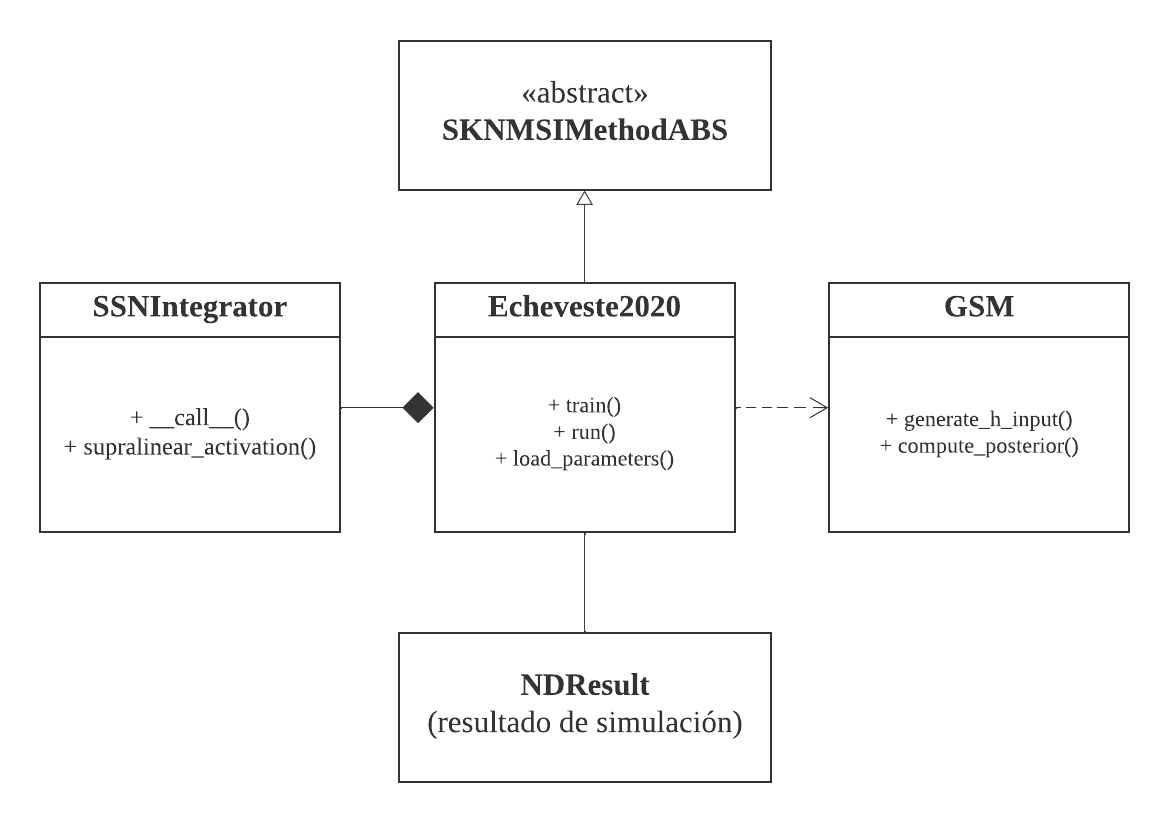
\includegraphics[width=0.8\textwidth]{07_implementacion/figures/DiagramaUML.png}
    \caption{Diagrama de clases UML simplificado de la implementación del modelo de Echeveste. Para una versión detallada, véase la Figura~\ref{fig:class-diagram}.}
    \label{fig:impl_clases}
\end{figure}

\subsection{Inicialización y configuración}
\label{subsec:impl_inicializacion}

El modelo por defecto se inicializa con parámetros nulos que deben ser optimizados antes de poder realizar inferencia. En este caso, el usuario debe invocar el método \texttt{train()} para ejecutar el procedimiento de optimización en dos etapas, o bien llamar al método \texttt{load\_parameters()} para cargar los parámetros pre-optimizados posteriormente. Una vez configurado el modelo, el método \texttt{run()} ejecuta la simulación de las dinámicas neuronales dado un estímulo especificado, retornando un objeto \texttt{NDResult} compatible con las herramientas de análisis del framework. El flujo completo de inicialización, entrenamiento y simulación se ilustra en detalle en el diagrama de secuencia en la Figura~\ref{fig:sequence-training-full}.

Otra opción es pasar el parámetro \texttt{pretrained=True} durante la construcción, esto cargará automáticamente los parámetros pre-optimizados por los autores originales, quedando listo para ejecutar simulaciones inmediatamente. Esta opción resulta conveniente para los usuarios que desean explorar el comportamiento del modelo sin invertir tiempo en el proceso de optimización.


% =============================================================================
% SECCIÓN 2: EL MODELO GENERATIVO GSM
% =============================================================================

\section{Implementación del modelo generativo}
\label{sec:impl_gsm}

El modelo generativo \acrshort{GSM} define el problema de inferencia que la red \acrshort{SSN} debe resolver. Desde el punto de vista de la implementación, cumple dos funciones esenciales: proporciona los estímulos de entrada transformados al espacio de la red neuronal y calcula los momentos objetivo contra los cuales se evalúa el desempeño durante el entrenamiento.

\subsection{Clase GSM y sus responsabilidades}
\label{subsec:impl_gsm_clase}

La clase \texttt{GSM} encapsula el modelo generativo descrito en la Sección~\ref{subsec:echeveste_gsm}. Sus responsabilidades principales incluyen la generación de filtros de Gabor que constituyen la matriz de campos proyectivos $\mathbf{A}$, la producción de parches de imagen con diferentes niveles de contraste según la Ecuación~\ref{eq:gsm}, el cálculo de la media y covarianza de la distribución posterior $P(\mathbf{y}|\mathbf{x}, z)$ según las Ecuaciones~\ref{eq:target_mean} y \ref{eq:target_cov}, y la aplicación de la transformación no lineal que convierte la proyección del estímulo en la entrada feedforward de las neuronas.

Una decisión de diseño importante fue separar la lógica del modelo generativo en una clase independiente, en lugar de integrarla directamente en la clase principal del modelo neuronal. Esta separación permite reutilizar el GSM en otros contextos, facilita las pruebas unitarias de cada componente, y refleja la distinción conceptual entre el problema computacional (definido por el GSM) y su implementación neuronal (la red SSN).

\subsection{Transformación de entrada feedforward}
\label{subsec:impl_gsm_h}

La transformación que convierte un parche de imagen $\mathbf{x}$ en la entrada feedforward $\mathbf{h}$ de la red neuronal es un punto crucial en nuestra implementación, siguiendo la Ecuación~\ref{eq:feedforward_input}. Esta transformación involucra tres parámetros optimizables ($\alpha_h$, $\beta_h$, $\gamma_h$) cuyos valores finales se presentan en la Tabla~\ref{tab:parametros_completos}.

La implementación sigue fielmente la formulación matemática, aplicando secuencialmente la proyección lineal mediante los pesos feedforward, el desplazamiento por la línea base, la rectificación, la potenciación, y finalmente el escalado. El valor del exponente $\gamma_h \approx 2$ resulta notablemente similar al exponente supralineal $n = 2$ utilizado en la función de transferencia de las neuronas, lo que sugiere una consistencia en el procesamiento no lineal a través del modelo.

% =============================================================================
% SECCIÓN 3: EL INTEGRADOR SSN
% =============================================================================

\section{Implementación del integrador SSN}
\label{sec:impl_ssn}

La base computacional del modelo es el integrador de la red supralineal estabilizada \acrshort{SSN}, que implementa las ecuaciones diferenciales que rigen la dinámica de los potenciales de membrana según la Ecuación~\ref{eq:ssn_dynamics}.

\subsection{Diseño de la clase}
\label{subsec:impl_ssn_integrador}

La clase \texttt{SSNIntegrator} se implementa como un \textit{dataclass} de Python que encapsula las ecuaciones diferenciales del modelo. Esta decisión de diseño tiene varias ventajas: permite que el mismo integrador sea reutilizado tanto durante el entrenamiento como durante la simulación, facilita su uso con el framework BrainPy para integración numérica, y hace explícitos los parámetros del modelo como atributos inmutables de la clase.

Los atributos de la clase corresponden a las constantes temporales de las poblaciones neuronales ($\tau_E$, $\tau_I$, $\tau_\eta$) y a los parámetros de la función de transferencia supralineal ($n$, $k$). Todos estos valores se mantienen fijos durante el entrenamiento según los valores de la Tabla~\ref{tab:parametros_completos}.

\subsection{Función de activación y ecuaciones dinámicas}
\label{subsec:impl_ssn_dynamics}

La función de transferencia supralineal convierte los potenciales de membrana en tasas de disparo según la Ecuación~\ref{eq:firing_rate}. La implementación utiliza el backend matemático de BrainPy, que permite ejecución transparente en GPU cuando está disponible, proporcionando aceleración significativa para simulaciones largas.

El método principal del integrador computa las derivadas temporales de los potenciales de membrana, manejando correctamente la estructura de bloques de la matriz de conectividad. Una consideración importante en la implementación es el respeto del principio de Dale: los signos de las conexiones están incorporados directamente en la matriz $\mathbf{W}$, de modo que las conexiones desde neuronas excitatorias son siempre positivas y las conexiones desde neuronas inhibitorias son siempre negativas.

% =============================================================================
% SECCIÓN 4: CONECTIVIDAD PARAMÉTRICA
% =============================================================================

\section{Conectividad paramétrica}
\label{sec:impl_conectividad}

Una característica distintiva del modelo de Echeveste es la parametrización circulante de la matriz de conectividad, que reduce drásticamente el número de parámetros libres respetando la simetría rotacional de la topología de anillo.

La matriz de conectividad $\mathbf{W}$ se construye a partir de solo 8 parámetros según la Ecuación~\ref{eq:weight_parametrization}. Esta parametrización reducida constituye una decisión de diseño fundamental del modelo. Con 100 neuronas en la red (50 excitatorias y 50 inhibitorias), una matriz de conectividad sin restricciones contendría 10,000 pesos sinápticos independientes. Optimizar tantos parámetros simultáneamente presentaría múltiples dificultades: el espacio de búsqueda sería enorme, el riesgo de sobreajuste a los estímulos de entrenamiento sería elevado, y el costo computacional de calcular gradientes para cada peso haría el entrenamiento impracticable.

La parametrización circulante resuelve estos problemas al explotar la simetría rotacional inherente a la topología de anillo. Dado que las neuronas están organizadas según su orientación preferida, resulta biológicamente plausible asumir que la fuerza de conexión entre dos neuronas depende únicamente de la diferencia entre sus orientaciones, no de sus valores absolutos. Esta suposición reduce drásticamente los grados de libertad: cada bloque de la matriz queda completamente determinado por solo dos parámetros, una amplitud $a$ y un ancho $d$, que definen un kernel gaussiano circular.

Cada uno de los cuatro bloques de la matriz ($\mathbf{W}_{EE}$, $\mathbf{W}_{EI}$, $\mathbf{W}_{IE}$, $\mathbf{W}_{II}$) se genera aplicando este kernel a las diferencias de orientación entre neuronas presinápticas y postsinápticas. El resultado es una matriz con estructura de banda: las conexiones son más fuertes entre neuronas con orientaciones similares y decaen suavemente para orientaciones distantes. Los valores optimizados de estos parámetros se presentan en la Tabla~\ref{tab:parametros_completos}.

La implementación construye cada bloque de manera vectorizada para mayor eficiencia computacional, evitando bucles explícitos sobre pares de neuronas. Esta vectorización resulta esencial dado que la construcción de la matriz debe realizarse múltiples veces durante el proceso de optimización, cada vez que se actualizan los parámetros de conectividad.

% =============================================================================
% SECCIÓN 5: PROCESO DE ENTRENAMIENTO
% =============================================================================

\section{Proceso de entrenamiento}
\label{sec:impl_entrenamiento}

El entrenamiento del modelo sigue el procedimiento de optimización en dos etapas descrito en la Sección~\ref{subsec:echeveste_entrenamiento}. La implementación utiliza JAX para diferenciación automática, combinando los optimizadores Optax (Stage 1) y SciPy (Stage 2). Para una visualización completa de las interacciones entre componentes durante ambas etapas de optimización, incluyendo el flujo de datos y las llamadas a funciones específicas, véase la Figura~\ref{fig:sequence-training-full}.

\subsection{Stage 1: Optimización estocástica con ADAM}
\label{subsec:impl_stage1}

La primera etapa utiliza el optimizador \acrshort{ADAM} con estimación estocástica de los momentos de respuesta. Los hiperparámetros de esta etapa están presentados en la siguiente tabla.

\begin{table}[H]
\centering
\caption{Hiperparámetros de optimización Stage 1.}
\label{tab:stage1_params}
\begin{tabular}{llc}
\toprule
\textbf{Parámetro} & \textbf{Descripción} & \textbf{Valor} \\
\midrule
$\eta$ & Tasa de aprendizaje ADAM & 0.002 \\
$\beta_1$ & Momento de primer orden & 0.9 \\
$\beta_2$ & Momento de segundo orden & 0.999 \\
$N_\text{trial}$ & Trials por iteración & 50 \\
Iteraciones & Número de pasos ADAM & 250 \\
\bottomrule
\end{tabular}
\end{table}

Una característica importante del Stage 1 es el  \textit{annealing} del tiempo inicial de integración $T_{\min}$, que comienza en 0 ms y aumenta progresivamente hasta $T_{\max} - 50$ ms a lo largo de las iteraciones. Este esquema de  \textit{curriculum learning} incentiva que la red aprenda dinámicas de muestreo rápidas desde el inicio del estímulo, evitando soluciones que solo convergen lentamente hacia los momentos objetivo.

\subsection{Stage 2: Optimización determinística con L-BFGS-B}
\label{subsec:impl_stage2}

La segunda etapa optimiza los 15 parámetros totales utilizando el optimizador quasi-Newton \acrshort{L-BFGS-B} con el método \acrshort{ADF} para calcular determinísticamente los momentos de respuesta. A diferencia del método estocástico de Stage 1 que puede tener alta varianza en las estimaciones, \acrshort{ADF} proporciona gradientes exactos (bajo la aproximación gaussiana) que permiten una convergencia más precisa.

Los parámetros adicionales optimizados en Stage 2 incluyen los 3 parámetros de la transformación de entrada ($\alpha_h$, $\beta_h$, $\gamma_h$) y los 4 parámetros de la covarianza de ruido ($\sigma_E$, $\sigma_I$, $\rho$, $d_\sigma$), cuyos valores óptimos se encuentran en la Tabla~\ref{tab:parametros_completos}.

\subsection{Función de costo}
\label{subsec:impl_costo}

La función de costo implementa la Ecuación~\ref{eq:cost_function}, penalizando diferencias entre los momentos de la distribución de respuestas de la red y los momentos objetivo del \acrshort{GSM}. Los pesos relativos de cada término, presentados en la siguiente tabla, fueron ajustados por los autores originales para balancear la contribución de cada componente.

\begin{table}[H]
\centering
\caption{Pesos de la función de costo.}
\label{tab:cost_weights}
\begin{tabular}{llc}
\toprule
\textbf{Peso} & \textbf{Término} & \textbf{Valor} \\
\midrule
$\epsilon_\mu$ & Error de media & $4.0 \times 10^{-5}$ \\
$\epsilon_\sigma$ & Error de varianza & $8.0 \times 10^{-5}$ \\
$\epsilon_\Sigma$ & Error de covarianza & $8.0 \times 10^{-7}$ \\
$\epsilon_{\text{slow}}$ & Penalización de lentitud & $4.0 \times 10^{-10}$ \\
\bottomrule
\end{tabular}
\end{table}

El término de \textit{slowness} penaliza la autocorrelación temporal de las respuestas, incentivando que muestras consecutivas sean estadísticamente independientes. Sin este término, la red podría aprender a producir los momentos correctos pero con dinámicas temporales excesivamente lentas que harían el muestreo ineficiente.

\subsection{Reimplementación en JAX}
\label{subsec:impl_jax}

Uno de los desafíos inesperados de este trabajo fue descubrir que el código de entrenamiento original de \citet{echeveste2020cortical} estaba implementado en OCaml\footnote{\url{https://ocaml.org/}}, un lenguaje de programación funcional que resulta completamente atípico para el desarrollo de modelos de redes neuronales en la actualidad. La comunidad de neurociencia computacional y aprendizaje automático ha convergido casi universalmente hacia Python como lenguaje de implementación, con frameworks como TensorFlow\footnote{\url{https://www.tensorflow.org/}}, PyTorch\footnote{\url{https://pytorch.org/}} o JAX\footnote{\url{https://docs.jax.dev/}} como herramientas estándar para diferenciación automática y cómputo en \acrshort{GPU}. Encontrar una implementación en OCaml representó un obstáculo considerable que requirió una adaptación drástica de nuestra estrategia de desarrollo.

En comunicación personal con el Dr. Echeveste, pudimos comprender las razones históricas detrás de esta elección. Dado el momento en que se desarrolló el modelo original (2016), las herramientas de diferenciación automática que hoy consideramos estándar no existían o no habían alcanzado la madurez necesaria para este tipo de aplicaciones. OCaml ofrecía entonces ciertas ventajas para implementar el método \acrshort{ADF}, que requiere propagar gradientes a través de ecuaciones diferenciales de manera eficiente. Sin embargo, esta decisión técnica, perfectamente razonable en su contexto original, dejó el código en un estado de difícil acceso para la comunidad científica actual.

La reimplementación en JAX constituyó, por tanto, no solo una traducción de código sino una actualización tecnológica sustancial del modelo. JAX fue la elección natural por varias razones. En primer lugar, su paradigma de programación funcional (con funciones puras, sin efectos secundarios ni estado mutable) guarda cierta afinidad conceptual con OCaml, lo que facilitó la traducción de las estructuras algorítmicas del código original. Las ecuaciones del modelo pueden expresarse en JAX de forma casi idéntica a su formulación matemática, manteniendo una correspondencia directa con el paper original.

En segundo lugar, JAX ya se encontraba integrado en el framework Scikit-NeuroMSI como dependencia para otros componentes. Esta preexistencia significó que los usuarios del framework no necesitan instalar dependencias adicionales para utilizar el modelo de Echeveste, y que la implementación puede beneficiarse de utilidades y patrones ya establecidos en el código base. Esta coherencia tecnológica dentro del framework simplifica el mantenimiento a largo plazo y facilita futuras integraciones entre modelos.

Desde el punto de vista computacional, JAX ofrece compilación \acrlong{JIT} mediante \acrshort{XLA}\footnote{
La compilación \acrshort{JIT} en JAX se basa en \acrfull{XLA}, un compilador que analiza el grafo completo de operaciones numéricas y produce una versión optimizada del cálculo, adaptada al dispositivo de ejecución, reduciendo el overhead interpretativo y el uso de memoria intermedia.
}
, que optimiza automáticamente las operaciones para el hardware disponible. Esto resulta particularmente beneficioso durante el entrenamiento, donde la función de costo y sus gradientes deben evaluarse cientos de veces. La transformación \texttt{jax.grad} permite obtener gradientes exactos de funciones arbitrarias de manera composicional: si una función $f$ se compone de operaciones diferenciables, su gradiente se obtiene automáticamente sin necesidad de derivar manualmente las expresiones analíticas. Esta capacidad es esencial para el método \acrshort{ADF} utilizado en Stage 2, donde los gradientes deben propagarse a través de la evolución temporal de los momentos de la distribución. Además, JAX proporciona soporte transparente para ejecución en \acrshort{GPU}, permitiendo acelerar significativamente tanto el entrenamiento como las simulaciones sin modificar el código.

En definitiva, la reimplementación en JAX transformó un código técnicamente correcto pero prácticamente inaccesible en una implementación moderna, mantenible y compatible con el ecosistema actual de herramientas de neurociencia computacional.

% =============================================================================
% SECCIÓN 6: SIMULACIÓN
% =============================================================================

\section{Simulación de dinámicas neuronales}
\label{sec:impl_simulacion}

Una vez entrenado el modelo (o cargados los parámetros pre-entrenados), el método \texttt{run()} ejecuta la simulación de las dinámicas neuronales. Esta sección describe los modos de simulación disponibles, el proceso de evolución temporal, y la estructura de los resultados.

\subsection{Modos de simulación}
\label{subsec:impl_modos}

La implementación soporta dos modos de simulación que corresponden a diferentes propósitos experimentales del trabajo original.

El \textbf{modo de fase única} (\textit{single-phase}) mantiene el estímulo presente durante toda la simulación. Este modo replica las condiciones utilizadas durante el entrenamiento de la red, donde la función objetivo evalúa las estadísticas de muestreo en estado estacionario. Es el modo apropiado para validar que la red entrenada reproduce correctamente las distribuciones \textit{target} del modelo \acrshort{GSM}, y para análisis de respuestas estacionarias como la sintonización de orientación y la variabilidad neural dependiente del contraste.

El \textbf{modo de tres fases} (\textit{three-phase}) divide la simulación en tres períodos temporales distintos: actividad espontánea pre-estímulo (225 ms por defecto), presentación del estímulo (100 ms), y actividad espontánea post-estímulo (125 ms). Este modo replica las condiciones experimentales del código de simulación original y permite estudiar fenómenos dinámicos que emergen específicamente del entrenamiento basado en muestreo: los \textit{overshoots} transitorios al inicio del estímulo, las dinámicas de \textit{onset/offset}, y las oscilaciones gamma moduladas por el estímulo.

El modo de tres fases soporta opcionalmente \textbf{delays por neurona} en las transiciones de estímulo, modelando la variabilidad temporal con que diferentes neuronas reciben la señal de entrada. Los delays se muestrean de una distribución normal con media de 45 ms y desviación estándar de 5 ms (valores por defecto del código original). Esta característica permite simular las condiciones utilizadas en el paper para analizar los \textit{overshoots} promediados sobre múltiples configuraciones de \textit{delay}.

La distinción entre ambos modos refleja un hallazgo central del trabajo original: aunque el entrenamiento optimiza para estado estacionario (modo single-phase), la red emergente exhibe dinámicas transitorias funcionalmente relevantes (modo three-phase). Los \textit{overshoots} al \textit{onset} del estímulo no son defectos sino características funcionales que mejoran la inferencia continua, compensando el sesgo introducido por promediar respuestas sobre ventanas temporales finitas \citep{echeveste2020cortical}.

\subsection{Evolución temporal e integración numérica}
\label{subsec:impl_evolucion}

El proceso de simulación consta de dos etapas: un período de estabilización inicial seguido del registro de actividad. La integración de las ecuaciones diferenciales (Ecuación~\ref{eq:ssn_dynamics}) utiliza el método de Euler explícito con paso de tiempo $dt = 0.2$ ms, consistente con el código original. El framework BrainPy proporciona la infraestructura de integración:

\begin{code}
\begin{minted}{python}
# Initialize BrainPy ODE integrator
integrator_model = SSNIntegrator(
    tau_e=0.020,  # 20 ms in seconds
    tau_i=0.010,  # 10 ms in seconds
    tau_n=0.020,  # 20 ms in seconds
    n=2.0, k=0.3
)
self._integrator = bp.odeint(f=integrator_model, method='euler', dt=0.2e-3)
\end{minted}
\caption{Inicialización del integrador numérico con BrainPy.}
\label{code:brainpy_integrator}
\end{code}
\vspace{1.5em}

La primera etapa es el período de \textbf{\textit{burn-in}}, durante el cual la red evoluciona sin registrar datos. Este período es necesario porque las condiciones iniciales (potenciales de membrana y ruido) se inicializan de manera arbitraria, y la red requiere tiempo para alcanzar el régimen estacionario estocástico desde el cual las muestras son representativas de la distribución posterior. El valor por defecto de 10,000 ms corresponde al utilizado en el código original, aunque para experimentos de transitorios se recomienda aumentarlo a 20,000 ms.

Durante tanto el burn-in como la simulación principal, el ruido de inferencia $\boldsymbol{\eta}$ evoluciona según un proceso que mantiene la estructura de correlaciones espaciales definida por la matriz $\boldsymbol{\Sigma}_\eta$:

\begin{code}
\begin{minted}{python}
def _update_noise(self, eta_old, L, dt, tau_n):
    """Update noise via Ornstein-Uhlenbeck process.
    
    η(t+dt) = η(t)·(1 - dt/τ_η) + √(2·dt/τ_η)·L·ξ
    where ξ ~ N(0,I) and L is Cholesky factor of Σ_η.
    """
    eps_1 = 1.0 - dt / tau_n
    eps_2 = np.sqrt(2.0 * dt / tau_n)
    xi = self._random.standard_normal(self._N)
    return eps_1 * eta_old + eps_2 * (L @ xi)
\end{minted}
\caption{Actualización del ruido correlacionado.}
\label{code:ou_noise}
\end{code}
\vspace{1.5em}

El loop principal de simulación alterna entre la actualización del ruido y la integración de las dinámicas neuronales, determinando el estímulo apropiado en cada paso según el modo de simulación y la fase temporal actual.

\subsection{Estructura del resultado}
\label{subsec:impl_resultado}

Una vez completada la evolución temporal, el método \texttt{run()} empaqueta las trayectorias registradas en un objeto \texttt{NDResult}, el formato estándar de resultados del framework. Esto permite que los resultados del modelo de Echeveste sean directamente compatibles con las herramientas de análisis y visualización desarrolladas para otros modelos del framework, facilitando comparaciones y análisis unificados. Pero a su vez, la complejidad de este nuevo modelo impulso el desarrollo de herramientas nuevas para su analisis las cuales se adaptaron y trabajan bajo este contexto para una mayor coherencia general.

En el caso de querer desarrollar o entender el codigo de analisis nuevo, es crucial comprender los \texttt{NDResult}, los cuales almacenan cuatro series temporales que capturan completamente el estado de la red durante la simulación. La variable \texttt{excitatory\_potential} contiene los potenciales de membrana $u_E(t)$ de las neuronas excitatorias, que son las variables dinámicas primarias de la Ecuación~\ref{eq:ssn_dynamics} cuyas fluctuaciones constituyen las muestras de la distribución posterior según la teoría de muestreo neural. La variable \texttt{inhibitory\_potential} almacena los potenciales de membrana $u_I(t)$ de las neuronas inhibitorias, esenciales para estabilizar la dinámica y generar las oscilaciones gamma características. Las variables \texttt{excitatory\_firing\_rate} e \texttt{inhibitory\_firing\_rate} contienen las tasas de disparo $r_E(t)$ y $r_I(t)$ respectivamente, calculadas aplicando la función de activación supralineal (Ecuación~\ref{eq:firing_rate}) a los potenciales de membrana. Estas tasas son directamente comparables con registros electrofisiológicos experimentales.

Cada serie temporal tiene dimensiones $(N_{\text{neurons}}, N_{\text{timesteps}})$, donde el número de pasos temporales depende de la duración de simulación y la resolución temporal. El objeto incluye además metadatos sobre los parámetros de simulación utilizados, permitiendo reproducibilidad completa de los resultados. El siguiente fragmento ilustra cómo acceder a los datos para análisis posteriores:

\begin{code}
\begin{minted}{python}
# Ejecutar simulación
result = model.run(stimulus_contrast=0.5, simulation_time=1000.0)

# Acceder a tasas de disparo excitatorias
r_e = result.e_.excitatory_firing_rate  # Shape: (50, 5000)

# Calcular media poblacional a lo largo del tiempo
mean_activity = r_e.mean(axis=0)  # Shape: (5000,)

# Obtener vector de tiempos
time_vector = result.times_  # Array de 0 a 1000 ms

# Usar herramientas del framework
result.plot.heatmap(mode='excitatory_firing_rate')
stats = result.stats.summary()
\end{minted}
\caption{Acceso a los datos de simulación mediante el objeto \texttt{NDResult}.}
\label{code:ndresult_access}
\end{code}
\vspace{1.5em}

Esta estructura unificada de resultados es particularmente relevante para el objetivo a largo plazo del proyecto: la integración del modelo de Echeveste con modelos de integración multisensorial como el de \citet{cuppini2017biologically}. Al compartir el mismo formato de salida, ambos modelos podrán ser analizados y comparados utilizando las mismas herramientas.

% =============================================================================
% SECCIÓN 7: MÓDULOS DE SOPORTE
% =============================================================================

\section{Módulos de soporte implementados}
\label{sec:impl_modulos_soporte}

Además de la implementación central del modelo de Echeveste, el presente trabajo contribuyó estructurando dos módulos completamente nuevos al framework Scikit-NeuroMSI: el módulo \texttt{data} para la gestión de datos pre-entrenados, y el módulo \texttt{generative} donde se encuentra nuestro modelo generativo. Estos módulos constituyen contribuciones a la arquitectura del framework, ampliando y generando una buena base para replicar en la implementación de futuros modelos.

\subsection{Cargadores de datos}
\label{subsec:impl_modulo_data}

El módulo \texttt{data} dentro del paquete \texttt{echeveste} fue implementado como una infraestructura completamente nueva para gestionar el acceso a datos pre-entrenados y configuraciones de modelos. Este diseño responde a la necesidad de separar claramente la lógica de carga de datos de la lógica de simulación, siguiendo el principio de responsabilidad única.

El módulo exporta dos clases principales. La clase \texttt{EchevesteDataLoader} proporciona acceso estructurado a todos los parámetros pre-entrenados del modelo de Echeveste, incluyendo la matriz de conectividad optimizada $\mathbf{W}$, la matriz de covarianza de ruido $\boldsymbol{\Sigma}_\eta$, los parámetros de transformación de entrada ($\alpha_h$, $\beta_h$, $\gamma_h$), y los parámetros de conectividad individuales ($a_{XY}$, $d_{XY}$). La clase \texttt{GSMDataLoader} gestiona el acceso a los componentes del modelo generativo \acrshort{GSM}, incluyendo los filtros de Gabor pre-entrenados (matriz $\mathbf{A}$), la matriz de covarianza \textit{a priori} $\mathbf{C}$, y los vectores de entrada $h$ pre-calculados para diferentes niveles de contraste.

Esta arquitectura de cargadores permite que los usuarios trabajen con el modelo sin necesidad de acceder directamente al sistema de archivos, proporcionando una interfaz programática limpia y validación automática de la integridad de los datos:

\begin{code}
\begin{minted}{python}
from skneuromsi.data import EchevesteDataLoader, GSMDataLoader

# Cargar parámetros de conectividad
loader = EchevesteDataLoader()
W_trained = loader.load_connectivity_matrix()
noise_cov = loader.load_noise_covariance()
input_params = loader.load_input_transformation_parameters()

# Cargar componentes del GSM
gsm_loader = GSMDataLoader()
gabor_filters = gsm_loader.load_gabor_filters()  # Shape: (256, 50)
prior_cov = gsm_loader.load_prior_covariance()   # Shape: (50, 50)
\end{minted}
\caption{Uso de los cargadores de datos implementados.}
\label{code:data_loaders}
\end{code}
\vspace{1.5em}

El método \texttt{load\_parameters()} de la clase \texttt{Echeveste2020} utiliza internamente el \texttt{Echeveste\allowbreak DataLoader} para configurar completamente el modelo con los parámetros pre-optimizados, dejándolo listo para ejecutar simulaciones inmediatamente. Esta funcionalidad resulta esencial para facilitar el uso del modelo sin necesidad de ejecutar el costoso proceso de entrenamiento.


\subsection{Nuevos tipos de modelos}
\label{subsec:impl_modulo_generative}

El módulo \texttt{generative} representa una extensión conceptual significativa del framework, introduciendo por primera vez la capacidad de definir modelos generativos que especifican el problema de inferencia que las redes neuronales deben resolver. Mientras que los modelos existentes en Scikit-NeuroMSI se enfocaban exclusivamente en la integración de señales sensoriales, este nuevo módulo permite definir distribuciones \textit{a priori} y calcular distribuciones posteriores que sirven como objetivos de entrenamiento.

Actualmente el módulo contiene la clase \texttt{GSM} que implementa el modelo de mezcla de escala gaussiana descrito en la Sección~\ref{subsec:echeveste_gsm}. Sin embargo, la arquitectura fue diseñada con extensibilidad en mente: futuros trabajos podrían agregar otros modelos generativos (como modelos de campo aleatorio de Markov, modelos de energía, o modelos generativos multimodales) siguiendo la misma interfaz, habilitando así el estudio de cómo diferentes supuestos generativos afectan las dinámicas de muestreo neural.

% =============================================================================
% SECCIÓN 8: INFRAESTRUCTURA DE VALIDACIÓN
% =============================================================================

\section{Infraestructura de validación}
\label{sec:impl_infraestructura}

La validación de la implementación requirió el desarrollo de una infraestructura complementaria para generar simulaciones sistemáticas y producir figuras comparativas con los resultados del artículo original. Esta infraestructura, aunque externa al paquete principal de Scikit-NeuroMSI, constituye una contribución importante del presente trabajo al permitir la reproducción rigurosa de los experimentos de \citet{echeveste2020cortical} y dichos resultados serán analizados en el Capítulo \ref{chapter:resultados}. 

\subsection{Pruebas unitarias y comparación con código original}
\label{subsec:impl_tests}

Se implementaron pruebas unitarias para verificar el comportamiento correcto de los componentes individuales, incluyendo la inicialización con parámetros por defecto, la verificación de valores correctos en la matriz de conectividad, el comportamiento de la función supralineal, y la reproducibilidad de resultados con semillas fijas.

Aunque el código original está escrito en OCaml, se realizaron comparaciones numéricas para verificar que los filtros de Gabor generados coinciden con los archivos proporcionados, que la matriz de conectividad construida desde parámetros reproduce fielmente la matriz pre-entrenada, y que los momentos posteriores del GSM coinciden para estímulos de prueba.

\subsection{Arquitectura de dos etapas para generación de figuras}
\label{subsec:impl_dos_etapas}

El flujo de trabajo para reproducir las figuras del artículo original se estructuró en dos etapas claramente separadas, siguiendo buenas prácticas de ingeniería de software para análisis reproducible.

La primera etapa consiste en la \textbf{generación de datos}: scripts ubicados en el directorio \texttt{figures/data/} ejecutan simulaciones con configuraciones específicas y almacenan los resultados en formato comprimido. Esta separación permite ejecutar simulaciones computacionalmente costosas una única vez y reutilizar los datos para múltiples análisis.

La segunda etapa consiste en la \textbf{generación de figuras}: scripts en directorios \texttt{figures/FigX/} (donde X corresponde al número de figura del artículo original) cargan los datos pre-generados y producen visualizaciones comparativas entre el observador ideal (\acrshort{GSM}) y la red neuronal (\acrshort{SSN}).

% La Figura~\ref{fig:impl_workflow} ilustra este flujo de trabajo:

% \begin{figure}[H]
%     \centering
%     \begin{tikzpicture}[
%         node distance=1.5cm,
%         box/.style={rectangle, draw, minimum width=3.5cm, minimum height=1cm, align=center, font=\small},
%         arrow/.style={->, thick, >=stealth}
%     ]

%     % Etapa 1: Generación de datos
%     \node[box, fill=blue!15] (sim) {Scripts de\\simulación};
%     \node[box, fill=green!15, right=2cm of sim] (data) {Banco de datos\\(\texttt{.npz}, \texttt{.json})};

%     % Etapa 2: Generación de figuras
%     \node[box, fill=orange!15, right=2cm of data] (viz) {Scripts de\\visualización};
%     \node[box, fill=red!15, right=2cm of viz] (figs) {Figuras\\comparativas};

%     % Flechas
%     \draw[arrow] (sim) -- node[above, font=\footnotesize] {ejecutar} (data);
%     \draw[arrow] (data) -- node[above, font=\footnotesize] {cargar} (viz);
%     \draw[arrow] (viz) -- node[above, font=\footnotesize] {generar} (figs);

%     % Etiquetas de directorio
%     \node[below=0.3cm of sim, font=\footnotesize\ttfamily] {figures/data/};
%     \node[below=0.3cm of data, font=\footnotesize\ttfamily] {simulations/};
%     \node[below=0.3cm of viz, font=\footnotesize\ttfamily] {figures/FigX/};

%     \end{tikzpicture}
%     \caption{Flujo de trabajo para generación de datos y figuras. La separación en dos etapas permite reutilizar simulaciones costosas para múltiples análisis.}
%     \label{fig:impl_workflow}
% \end{figure}

El script principal \texttt{generate\_simulations.py} ejecuta simulaciones para los cinco niveles de contraste del conjunto de entrenamiento original ($z \in \{0,\allowbreak 0.125,\allowbreak 0.25,\allowbreak 0.5,\allowbreak 1.0\}$) con una configuración unificada. Para cada nivel de contraste, el script instancia el modelo, carga los parámetros pre-entrenados, ejecuta la simulación, calcula estadísticas del estado estacionario, y almacena las trayectorias temporales y estadísticas en formato NumPy comprimido (\texttt{.npz}) junto con metadatos en formato JSON para trazabilidad.

Esta infraestructura permite no solo validar la implementación contra los resultados publicados, sino también explorar configuraciones alternativas de manera sistemática y reproducible.

% =============================================================================
% SECCIÓN 9: REFERENCIA DE PARÁMETROS
% =============================================================================

\section{Referencia de parámetros}
\label{sec:impl_parametros}

A modo de referencia, la Tabla~\ref{tab:parametros_completos} consolida todos los parámetros del modelo descritos a lo largo de este capítulo, distinguiendo entre aquellos que permanecen fijos durante el entrenamiento y aquellos que son optimizados. Esta tabla corresponde a la Tabla Suplementaria S1 del artículo original \citep{echeveste2020cortical}. Los valores optimizados corresponden a los obtenidos por los autores tras el procedimiento de entrenamiento en dos etapas, y están disponibles en nuestra implementación mediante el método \texttt{load\_parameters()}.

\begin{table}[!ht]
\centering % Este comando centra la tabla
\caption{Parámetros completos del modelo de \citeauthor{echeveste2020cortical}, correspondientes a la Tabla Suplementaria S1 del artículo original.}
\label{tab:parametros_completos}
\makebox[\textwidth][c]{% Este comando fuerza el centrado respecto al papel
\begin{tabular}{llcc}
\toprule
\textbf{Categoría} & \textbf{Parámetro} & \textbf{Símbolo} & \textbf{Valor} \\
\midrule
\multirow{\textbf{Red neuronal (fijos)}} 
    & Neuronas excitatorias & $N_E$ & 50 \\
    & Neuronas inhibitorias & $N_I$ & 50 \\
    & Constante de tiempo E & $\tau_E$ & 20 ms \\
    & Constante de tiempo I & $\tau_I$ & 10 ms \\
    & Constante de tiempo ruido & $\tau_\eta$ & 20 ms \\
    & Exponente supralineal & $n$ & 2.0 \\
    & Factor de escala & $k$ & 0.3 \\
\midrule
\multirow{\textbf{Modelo GSM (fijos)}} 
    & Número de píxeles & $N_x$ & 256 \\
    & Número de orientaciones & $N_y$ & 50 \\
    & Desv. estándar ruido píxel & $\sigma_x$ & 10.0 \\
    & Factor escala $\mathbf{W}^{ff}$ & --- & $1/15$ \\
\midrule
\multirow{\textbf{Conectividad (optimizados)}} 
    & Amplitud E$\rightarrow$E & $a_{EE}$ & 1.46 \\
    & Amplitud E$\rightarrow$I & $a_{EI}$ & 1.29 \\
    & Amplitud I$\rightarrow$E & $a_{IE}$ & $-$1.96 \\
    & Amplitud I$\rightarrow$I & $a_{II}$ & $-$1.21 \\
    & Ancho E$\rightarrow$E & $d_{EE}$ & 0.56 \\
    & Ancho E$\rightarrow$I & $d_{EI}$ & 0.56 \\
    & Ancho I$\rightarrow$E & $d_{IE}$ & 0.40 \\
    & Ancho I$\rightarrow$I & $d_{II}$ & 0.40 \\
\midrule
\multirow{\textbf{Covarianza ruido (optimizados)}} 
    & Desv. estándar ruido E & $\sigma_E$ & 2.80 \\
    & Desv. estándar ruido I & $\sigma_I$ & 1.60 \\
    & Correlación E-I & $\rho$ & 0.75 \\
    & Ancho correlación & $d_\sigma$ & 0.45 \\
\midrule
\multirow{\textbf{Entrada (optimizados)}} 
    & Escala entrada & $\alpha_h$ & 1.96 \\
    & Línea base entrada & $\beta_h$ & 0.10 \\
    & Exponente entrada & $\gamma_h$ & 2.03 \\
\bottomrule
\end{tabular}

}
\end{table}


% =============================================================================
% SECCIÓN 10: RESUMEN DEL CAPÍTULO
% =============================================================================

\section{Resumen del capítulo}
\label{sec:impl_resumen}

Este capítulo presentó la implementación completa del modelo de \citeauthor{echeveste2020cortical} dentro del framework Scikit-NeuroMSI, junto con la infraestructura de soporte necesaria para su validación. Los principales aportes incluyen una arquitectura modular que separa claramente el modelo generativo \acrshort{GSM}, el integrador de dinámicas (\texttt{SSNIntegrator}), y la clase principal (\texttt{Echeveste2020}); la implementación del procedimiento de optimización en dos etapas usando \acrshort{ADAM} y \acrshort{L-BFGS-B} con \acrshort{ADF}; y la compatibilidad total con el framework mediante herencia de la clase base abstracta.

Como contribuciones adicionales al framework, se desarrolló el módulo \texttt{data} con una nueva infraestructura de cargadores que proporciona acceso estructurado a los parámetros pre-entrenados y componentes del modelo generativo, y el módulo \texttt{generative} que introduce por primera vez modelos generativos como el \acrshort{GSM}, permitiendo definir distribuciones \textit{a priori} y calcular los momentos posteriores que sirven como objetivos de entrenamiento. Este último módulo fue diseñado con extensibilidad en mente para incorporar futuros modelos generativos.

La reimplementación en JAX transformó el código original en OCaml en una implementación moderna con soporte para aceleración en \acrshort{GPU}. La infraestructura de validación desarrollada, basada en un sistema de dos etapas para generación de datos y visualización, permite ejecutar simulaciones sistemáticas y producir figuras comparativas de manera reproducible. Los resultados detallados de estas comparaciones se presentan en el Capítulo~\ref{chapter:resultados}, donde se analiza la concordancia entre los momentos de respuesta de la red y los objetivos del modelo generativo, las estructuras de correlación, y las propiedades dinámicas emergentes.